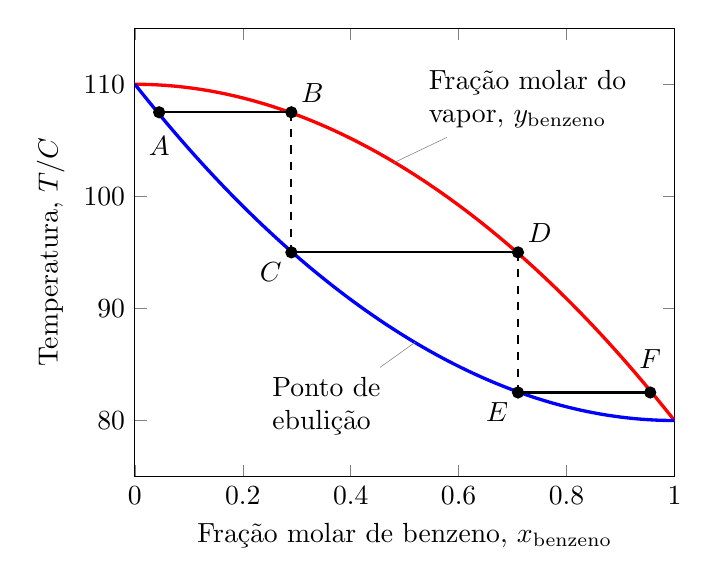
\begin{tikzpicture}
\begin{axis}
    [
        grid = minor,
        xlabel = {Fração molar de benzeno, $x_\mathrm{benzeno}$},
        ylabel = {Temperatura, $T/\unit{\degree C}$},
        xmin = 0, xmax = 1,
        ymin = 75, ymax = 115,
    ]    
            
    \draw [draw=red, very thick]
        (axis cs: 0, 110) parabola bend  (axis cs: 0, 110)
        (axis cs: 1, 80);

    \draw [draw=blue, very thick]
        (axis cs: 0, 110) parabola bend  (axis cs: 1, 80)
        (axis cs: 1, 80);

    \addplot [ mark=*, color=black, only marks ] coordinates
        {
            (0.045, 107.5)
            (0.290, 107.5)
            (0.290, 95)
            (0.710, 95)
            (0.710, 82.5)
            (0.955, 82.5)
        };

    \draw [draw=black, thick] (0.045, 107.5) -- (0.290, 107.5);
    \draw [draw=black, thick, dashed] (0.290, 107.5) -- (0.290,  95.0);
    \draw [draw=black, thick] (0.290,  95.0) -- (0.710,  95.0);
    \draw [draw=black, thick, dashed] (0.710,  95.0) -- (0.710,  82.5);
    \draw [draw=black, thick] (0.710,  82.5) -- (0.955,  82.5);

    \node[coordinate, pin={[fill=white, align=left] below left:{Ponto de\\ebulição}}] 
        at (axis cs:0.52, 87) {};

    \node[coordinate, pin={[fill=white, align=left] above right:{Fração molar do\\ vapor, $y_\mathrm{benzeno}$}}] 
        at (axis cs:0.48, 103) {};

    \node [anchor = north, inner sep=2ex] at (axis cs:0.045, 107.5) {$A$};
    \node [anchor = south west] at (axis cs:0.290, 107.5) {$B$};
    \node [anchor = north east] at (axis cs:0.290, 95) {$C$};
    \node [anchor = south west] at (axis cs:0.710, 95) {$D$};
    \node [anchor = north east] at (axis cs:0.710, 82.5) {$E$};
    \node [anchor = south, inner sep=2ex] at (axis cs:0.955, 82.5) {$F$};
        
\end{axis}
\end{tikzpicture}